\title{Opportunities for open-source software to accelerate research in applied geophysics}

\begin{abstract}
This article considers the potential for open-source software and open-science practices to accelerate research in applied geophysics and thereby contribute to solutions of geoscientific problems impacting society. We provide context on the definition of open-source and give a brief history of open-source software in applied geophysics. Drawing from our experience in the SimPEG project, which develops software for simulation and inversion of geophysical data, we provide two examples where research was accelerated because of open-source software. These include the re-use of regularization methods for different geophysical problems (magnetics and time-domain electromagnetics), and the combination of multiple geophysical data types in joint inversions. We also provide an example where research code was re-purposed for education and humanitarian projects. Each of these examples was made possible because of the availability of code and the practices adopted by the community of collaborators involved in the project. We conclude with our perspective on how practices adopted by open-source communities that enable collaboration amongst researchers with different backgrounds, skills, and interests can be applied more broadly in research. This will ultimately increase the use and effectiveness of geophysics in helping solve applied problems.
\end{abstract}

\section{Introduction and Motivation}
This special issue discusses several pressing applications where geophysics has an important role to play in non-invasively imaging the subsurface. These societal problems include locating critical minerals for transition to an electric economy, finding and managing our groundwater resources, sequestering  CO$_2$ to prevent more warming of the planet, and further developing other more sustainable sources of energy (geothermal, wind, solar, etc). \cite{capello_presidents_2022} provides a vision of how geophysics can have an impact on the United Nations' sustainable development goals. The problems to be addressed are complex and multidisciplinary. Their solutions require observational data, computational methods for working with those data, and interaction between researchers with a range of backgrounds and skills. Our hypothesis is that research in applied geophysics to help reach solutions to these problems can be accelerated by adopting open-source practices in the way we conduct research.

Applied problems are intrinsically multi-disciplinary and their solution requires input from many different disciplines. Geophysics can provide important information but its effectiveness can be realized only when we connect with other disciplines. The first connection point requires that we be able to pose the question at hand in terms of relevant physical properties. This could entail collaborating with a geologist to build a conceptual ore-deposit model for mineral exploration or connecting with a geochemist to characterize how physical properties change as CO$_2$ is injected and reacts with the surrounding formation or fluids. Once data have been collected, we then aim to interpret those data in light of the original question. In this stage, we are faced with the challenges that are inherent with any inverse problem, particularly, that solutions are non-unique. Additional data and a-priori information can help constrain a solution or interpretation. This again requires communication between practitioners in multiple fields but also requires tools at the computational level to bring in data and information in a quantitative manner. This is especially relevant with advances in machine learning that enable a wide array of data types to be analyzed and combined. Improvements in efficiency and effectiveness in the communication of information and data between disciplines, alongside advancements within each discipline, can help contribute to accelerating discovery.

Science advances by building upon ideas and each other's work. Open-source software enables us to build upon and extend prior work in a very tangible way. In addition to the lines of code, there are practices that have been adopted by many projects to help facilitate collaboration among researchers. Practices such as testing code and peer review of work enable multiple people to work on a common project, and having open discussions about challenges to overcome or new ideas to implement supports the building of connections between researchers from a variety of backgrounds. With computation and scientific software being such an essential part of research in applied geophysics, we see opportunities for open-source software, and more broadly, open science practices, to accelerate research within geophysics and broaden the impact of our work.

\begin{figure}[!htb]
    \begin{center}
    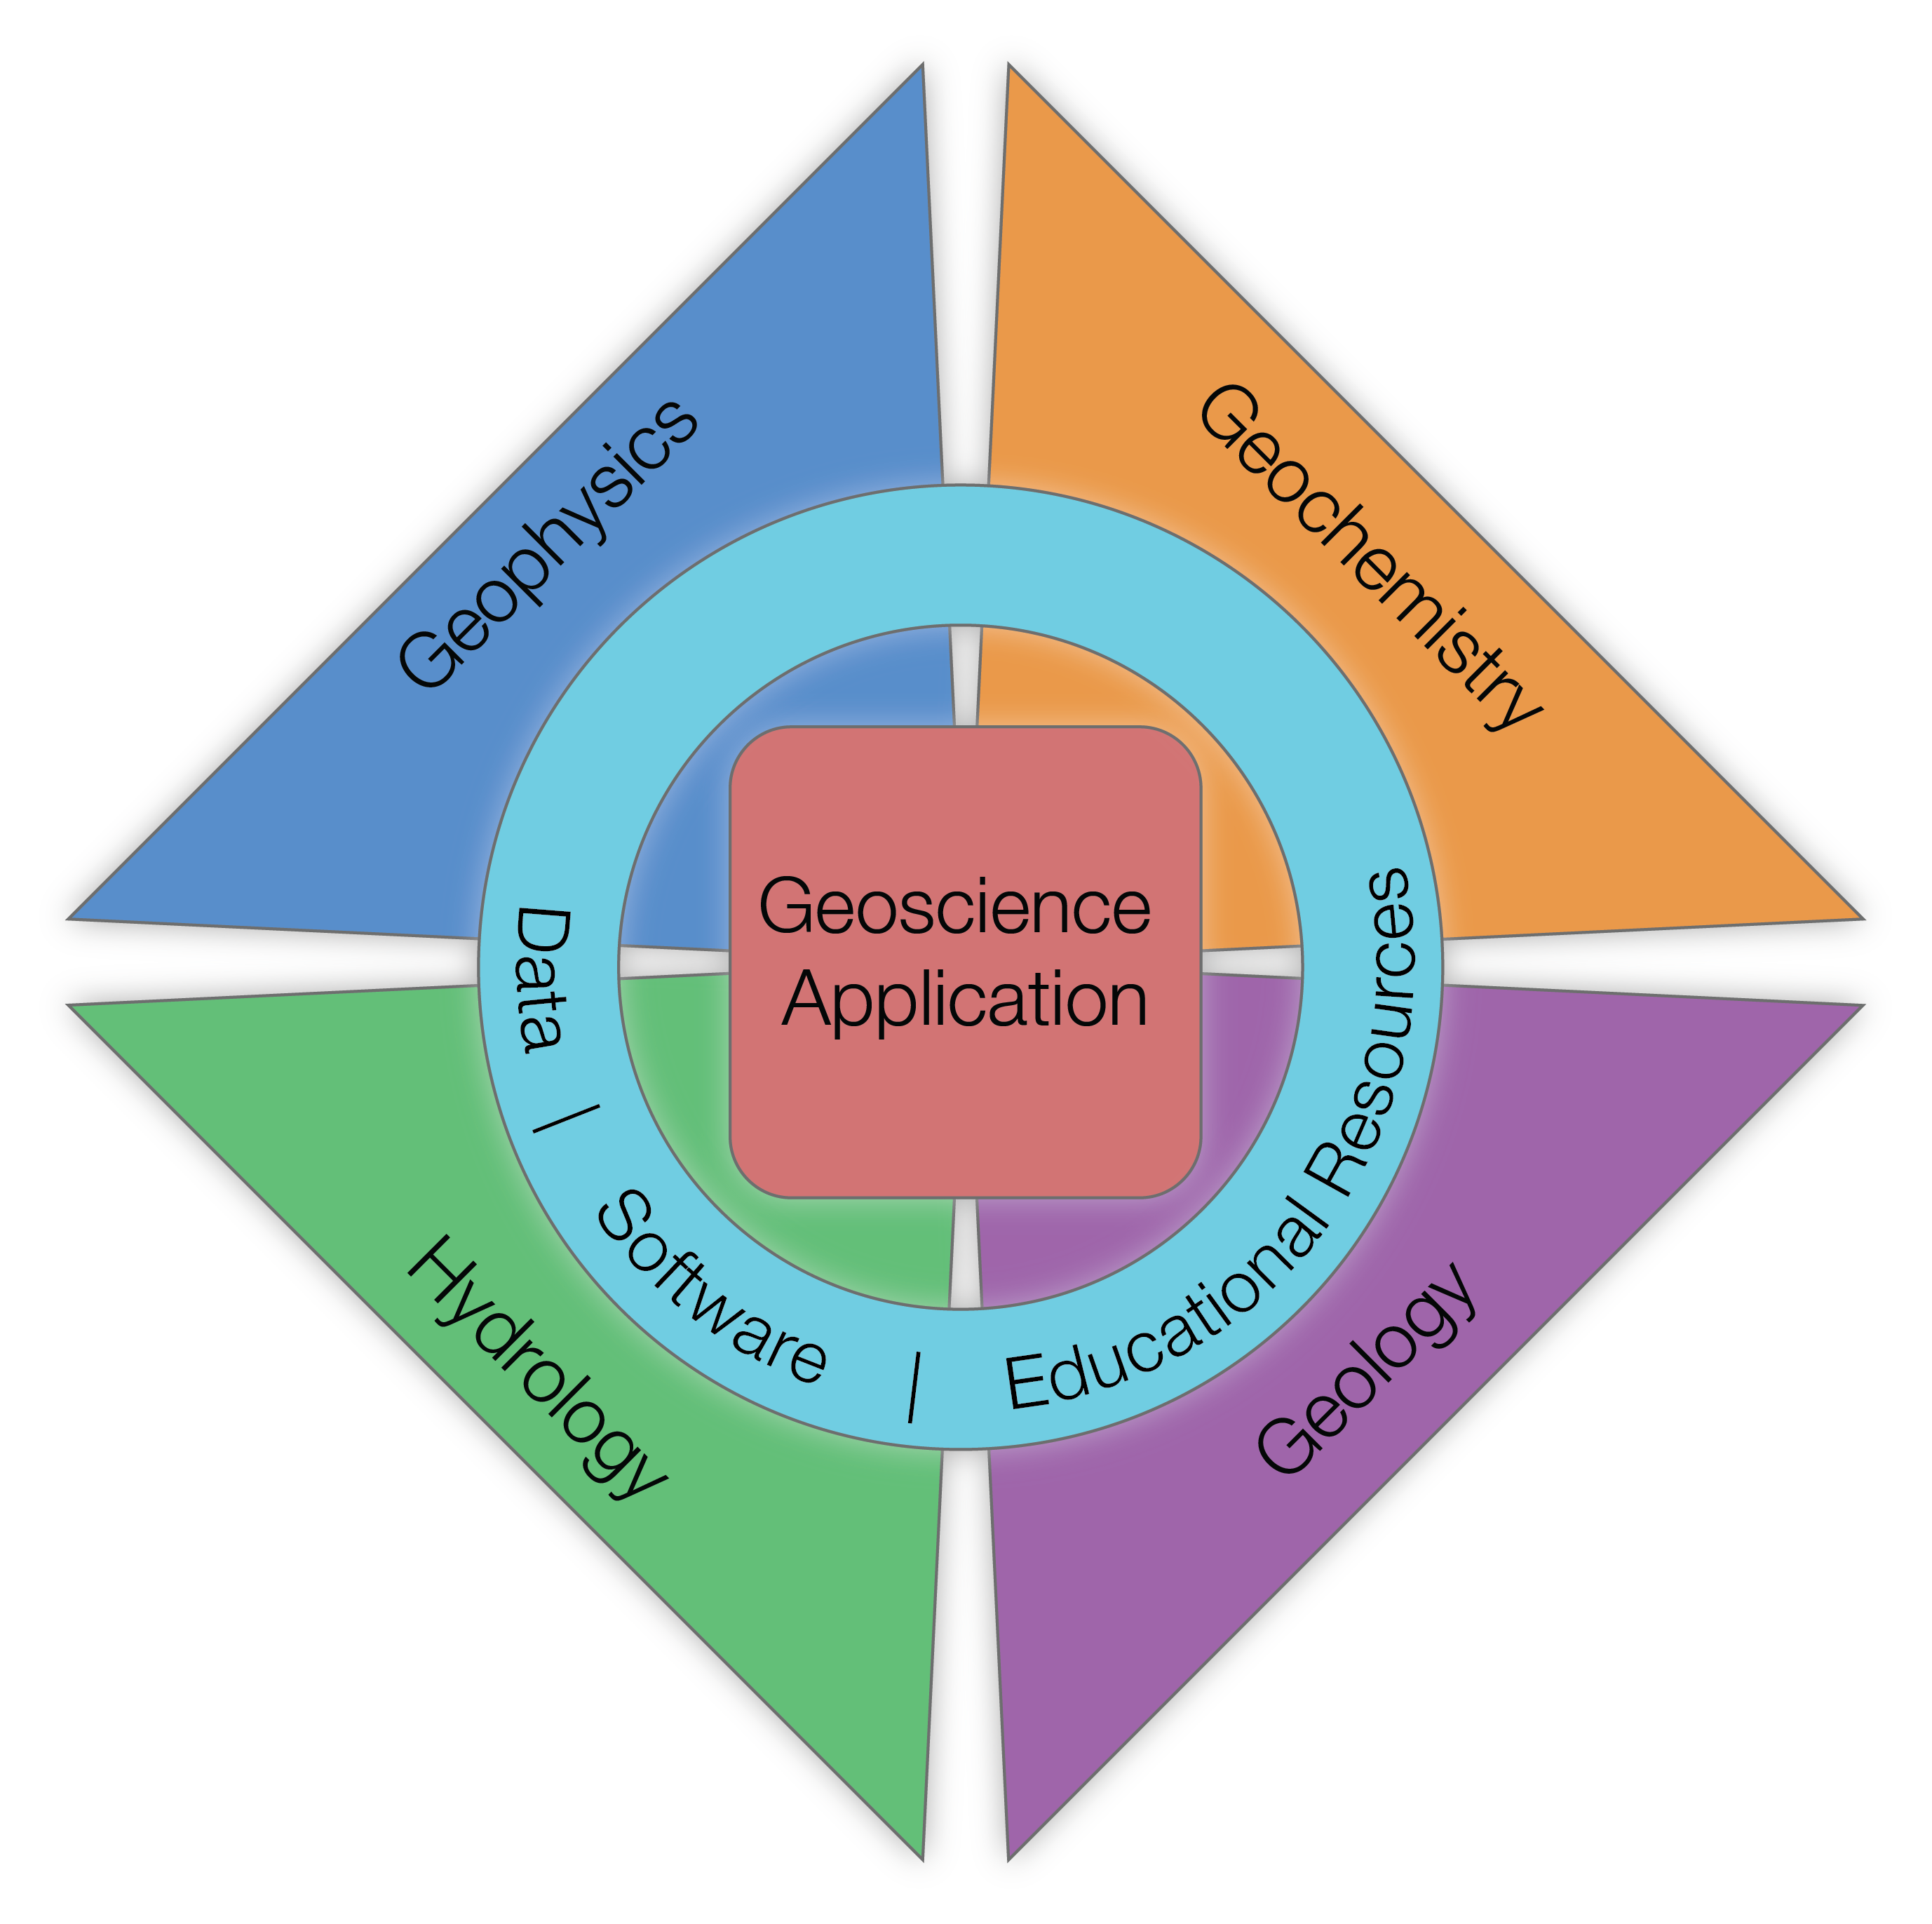
\includegraphics[width=0.55\textwidth]{figures/pizza-box.png}
    \end{center}
\caption{
     Any application requires perspectives and input from multiple disciplines. Data, software, and educational resources can help provide a bridge between disciplines. After \citep{oldenburg_3d_2020}
}
\label{fig:pizza-box}
\end{figure}


In this article, we illustrate that open-source software and practices can accelerate the exchange of ideas and facilitate collaborations between researchers. We will provide some background and context about open-source software in geophysics and illustrate examples of impacts in research based on our experience in developing and contributing to SimPEG, an open-source project for simulation and inversion of geophysical data.

\section{Background: Open-source software}

Before making an argument for open-source software, we begin by defining what we mean by ``open-source''. The Open Source Initiative (OSI) is a non-profit organization that maintains the Open Source Definition which specifies 10 criteria for a software project to be considered open-source. Source code must be accessible, and importantly, the license that is used must allow for the use, adaptation, and redistribution of the original or derived works. The criteria also specify that the license should not discriminate against use by any group or for any field of application. The full terms of the definition can be viewed at: \href{https://opensource.org/definition-annotated}{https://opensource.org/definition-annotated}.

Broadly speaking, there are two categories of open-source licenses: copyleft licenses and permissive licenses. Copyleft licenses, such as the GNU General Public License (GPL), require any derived works to also be distributed with the same license. Permissive licenses allow derived works to be distributed as open or closed software. Common examples of permissive licenses include the MIT license, BSD licenses, and Apache licenses. Within the scientific Python community, permissive licenses have been widely adopted. This choice has helped facilitate connections and collaboration amongst open-source developers and commercial entities by enabling the redistribution of code for commercial purposes. There are many great resources including \href{https://choosealicense.com}{https://choosealicense.com} and \href{https://opensource.org}{https://opensource.org}  that provide further background on software licenses for the interested reader.


\section{Brief overview of open-source in applied geophysics}

Distributing software with an open-source license is not a new concept in geophysics. Seismic Un*x (SU \cite{stockwell_cwpsu_1999}) was started in the 70's. In addition to being a useful codebase, the project also was important in demonstrating how open-source codes can facilitate computational reproducibility \citep{Claerbout1992}, that is, the ability to consistently obtain the same results using the same input data and computational methods as were used by the original authors. Other early open-source projects in and related to geophysics include MODFLOW for simulating groundwater flow \cite{langevin_modflow_2017}, Occam 1D for inverting controlled source electromagnetics (CSEM) and magnetotelluric (MT) data in 1D \cite{constable_occams_1987}, and Generic Mapping Tools (GMT) for plotting and visualizing geospatial data. Community mailing lists and websites such as MTNet provided avenues for distributing these codes. These codes continue to be maintained and widely used.

\begin{figure}[!htb]
    \begin{center}
    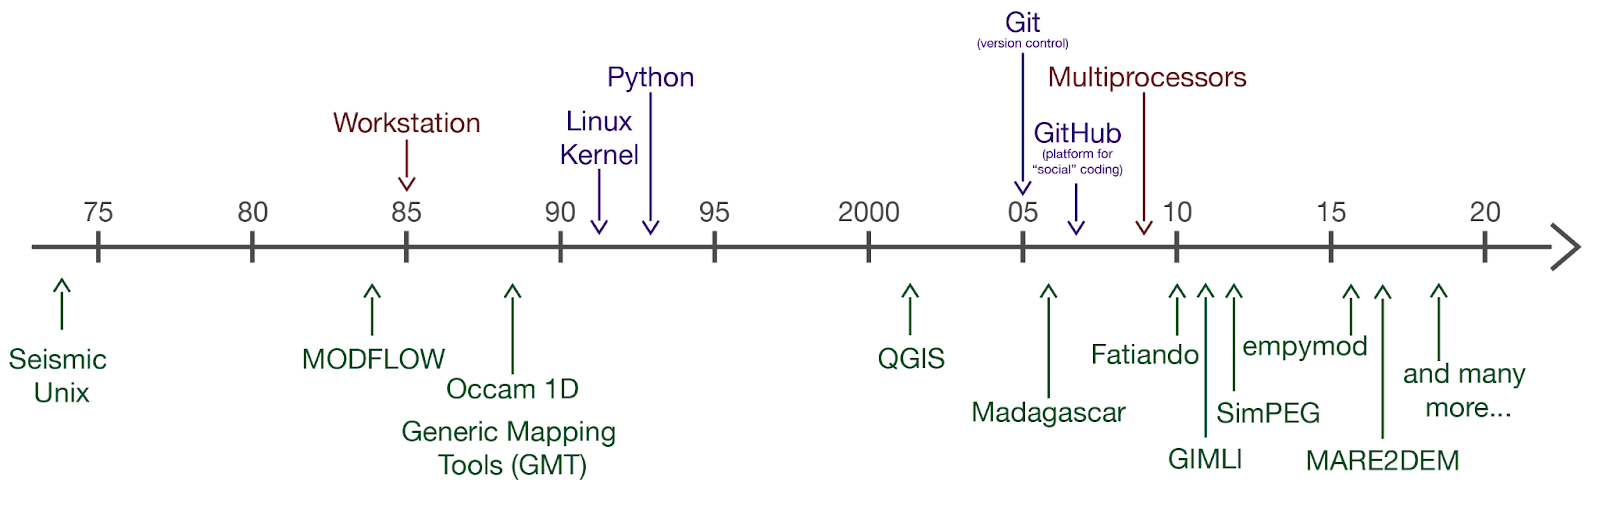
\includegraphics[width=\textwidth]{figures/oss-timeline.png}
    \end{center}
\caption{
    A sampling of open-source projects in geophysics through time.
}
\label{fig:oss-timeline}
\end{figure}


Several key developments have catalyzed the proliferation of open-source software packages we see in geophysics today. In the early 90's the first version of the Linux kernel was released providing the basis for many operating systems used in scientific computing (and elsewhere). The Python language was also started in the 90's, followed by Julia, R, and others. These languages are interpreted languages, as compared to Fortran and C which are compiled, and are arguably much easier to write scientific code with. The ability to rapidly write useable code is further aided by the existence of packages such as Numpy, Scipy, and Matplotlib, which provide useful functions for scientific computing. These components provide a base layer for the open-source scientific ``stack'', on top of which other projects can be built.

The next key developments were version control and platforms that provide infrastructure for collaborating on code. The combination of distributed version control with Git, and cloud-hosted platforms like GitHub for managing Git repositories, enables collaboration on code and facilitates software engineering practices. Having a forum to discuss issues or changes to the code, infrastructure to automatically run a test suite on a code base, tools for packaging and distributing code as well as for launching web-based documentation, enable collaboration amongst researchers and support the development of communities around these projects. These tools and practices have all contributed to the growth of what we now consider the modern open-source ecosystem.

In addition to enabling technologies, there are also social driving factors. These are illustrated by the renewed discussions on reproducibility and replicability in science, particularly in computational work \citep{national_academies_of_sciences_reproducibility_2019}, as well as the establishment of principles such as the FAIR (Findable, Accessible, Interoperable and Reusable) for scientific data management. Contributing to open-source software can also be an avenue for individuals to advance their career and profile; many researchers now list open-source projects that they contribute to in their CV or include links to sources such as a GitHub profile that show contributions through time. This is further evidence that open-source software is a valued part of the scientific conversation.

Much progress has been made in the open-source community and we are now at a point where you can find open-source software packages in nearly every field, and for a wide range of specialized tasks. There are even open-source projects to help navigate the available software for various scientific domains, including in the geosciences \cite{awesome-open-geoscience}.


\section{Impacts of open-source software in applied geophysics}

Assessing the ``impact'' of scholarly outputs, whether papers, software, data or otherwise, is a challenging objective and there are a variety of strategies that can be adopted. Quantitative metrics such as number of citations or downloads can provide an indication. There are also some studies that have sought to quantify the economic impacts of open-source software on jobs and GDP \citep{european_commission_impact_2021}. In what follows, we use examples to illustrate how open-source software can impact research. Rather than making an argument based on some metric for the value of open-source, our goal is to spark ideas for where, and how, researchers can have an impact by adopting open-source practices.

Looking to other fields, we can see some places where the use of open-source software has become a standard. Notably, much of the growth of machine learning (ML) research has been facilitated by tools like Scikit-learn, Pytorch, and Tensorflow that provide a base layer for that research. Additionally, it has become more the norm rather than the exception that code is made available with publications in ML research. Neural networks can be complex, and even with a well-written methods section in a paper, it is generally not straightforward to reproduce and extend work. Seeing the code authors have written (even if it is messy!) provides a starting point and can save time that would have otherwise been spent re-inventing the same work.

Having access to source code to reproduce a given result is particularly important in methods-oriented research where the approach for solving a problem is the scientific contribution. This is true when designing a neural network, and when simulating complex equations or solving inverse problems in geophysics. Inverse problems in particular are inherently non-unique and the solution that is obtained depends upon the implementation and the choices made by the user.

There are multiple open-source projects for simulating and inverting geophysical data (e.g. \cite{key_mare2dem_2016, Rucker2017, blanchy_resipy_2020, biondi_object-oriented_2021, mardan_pyfwi_2023}), and for working with geophysical data more broadly (e.g. \cite{Uieda2013, krieger_mtpy_2014, stanton_seismic_2016, warren_gprmax_2016, louboutin_devito_2019}). Each of these projects undoubtedly has examples that could be shared that illustrate impacts on research in geophysics. Our focus in the following sections is on SimPEG because it is the project that we work on and have context with.

We started the SimPEG project to develop a framework and toolbox for solving inverse problems in geophysics \cite{cockett_simpeg_2015}. Promoting transparency \& reproducibility, facilitating collaboration, and enabling researchers to rapidly experiment with the work of others were prime motivating factors to start SimPEG as an open-source project. In the following material, we illustrate some of the ways in which we have seen research accelerated because of the open-source principles and practices used within the SimPEG community.


\subsection{Accelerated research, education, and outreach in the SimPEG community}

SimPEG solves finite-volume numerical simulations and gradient-based inversions. It uses the permissive MIT license which allows for academic and commercial use and adaptation. It is designed to be modular so that pieces can be interchanged and extended independently of each other but be able to work together.

The general inverse problem solved by SimPEG is an optimization problem that is comprised of a data misfit ($\phi_d$) and a regularization term ($\phi_m$) with a trade-off parameter ($\beta$) between them, as shown in equation \ref{eq:inverse-problem}
\begin{equation}
\underset{m}{\text{minimize}} ~ \phi(m) = \phi_d(m) + \beta\phi_m(m)
\quad \text{s.t.}~\phi_d \leq \phi_d^*
\label{eq:inverse-problem}
\end{equation}

Solving this problem requires the ability to simulate geophysical data, compute sensitivities with respect to model parameters, define a regularization, and implement heuristics such as a $\beta$-cooling strategy to obtain a solution that fits the data \citep{Oldenburg2005}.

A conceptual diagram that illustrates how we organize the components of the inverse problem is shown in Figure \ref{fig:simpeg-framework}. The measured data, an estimate of the uncertainties, knowledge of the governing physical equations, and a priori information and assumptions about the geologic question are inputs to the inversion. In the implementation, we then arrange the various components as modules that are combined to solve the inverse problem. First, we need a mechanism to simulate data, for this, we take a finite-volume approach, meaning that a \textbf{Mesh} (e.g. a Tensor or OcTree mesh) is designed and provided to the \textbf{Simulation}, which has the necessary components to solve the equations of interest (e.g. time-domain electromagnetics or gravity). The \textbf{Survey} contains the information about the sources and receivers (type and locations) that are employed. With this information provided, we can then simulate predicted data. Note that the \textbf{Simulation} also contains machinery to compute sensitivities (or products of a vector with the sensitivity) for gradient-based optimization.

To perform the inversion, we then define the observed \textbf{Data} and construct the \textbf{Data Misfit} and \textbf{Regularization} terms that are combined to define the define the objective function for the \textbf{Inverse Problem} (equation \ref{eq:inverse-problem}). We choose an \textbf{Optimization} strategy that will be used for minimizing the objective function (e.g. Inexact Gauss Newton). The \textbf{Inversion} module brings together all of these components along with additional instructions (that are called \textbf{Directives} in SimPEG), such as the use of a $\beta$-cooling schedule or a stopping criteria based on a target misfit value, that are enacted when the inversion is run.

\begin{figure}[!htb]
    \begin{center}
    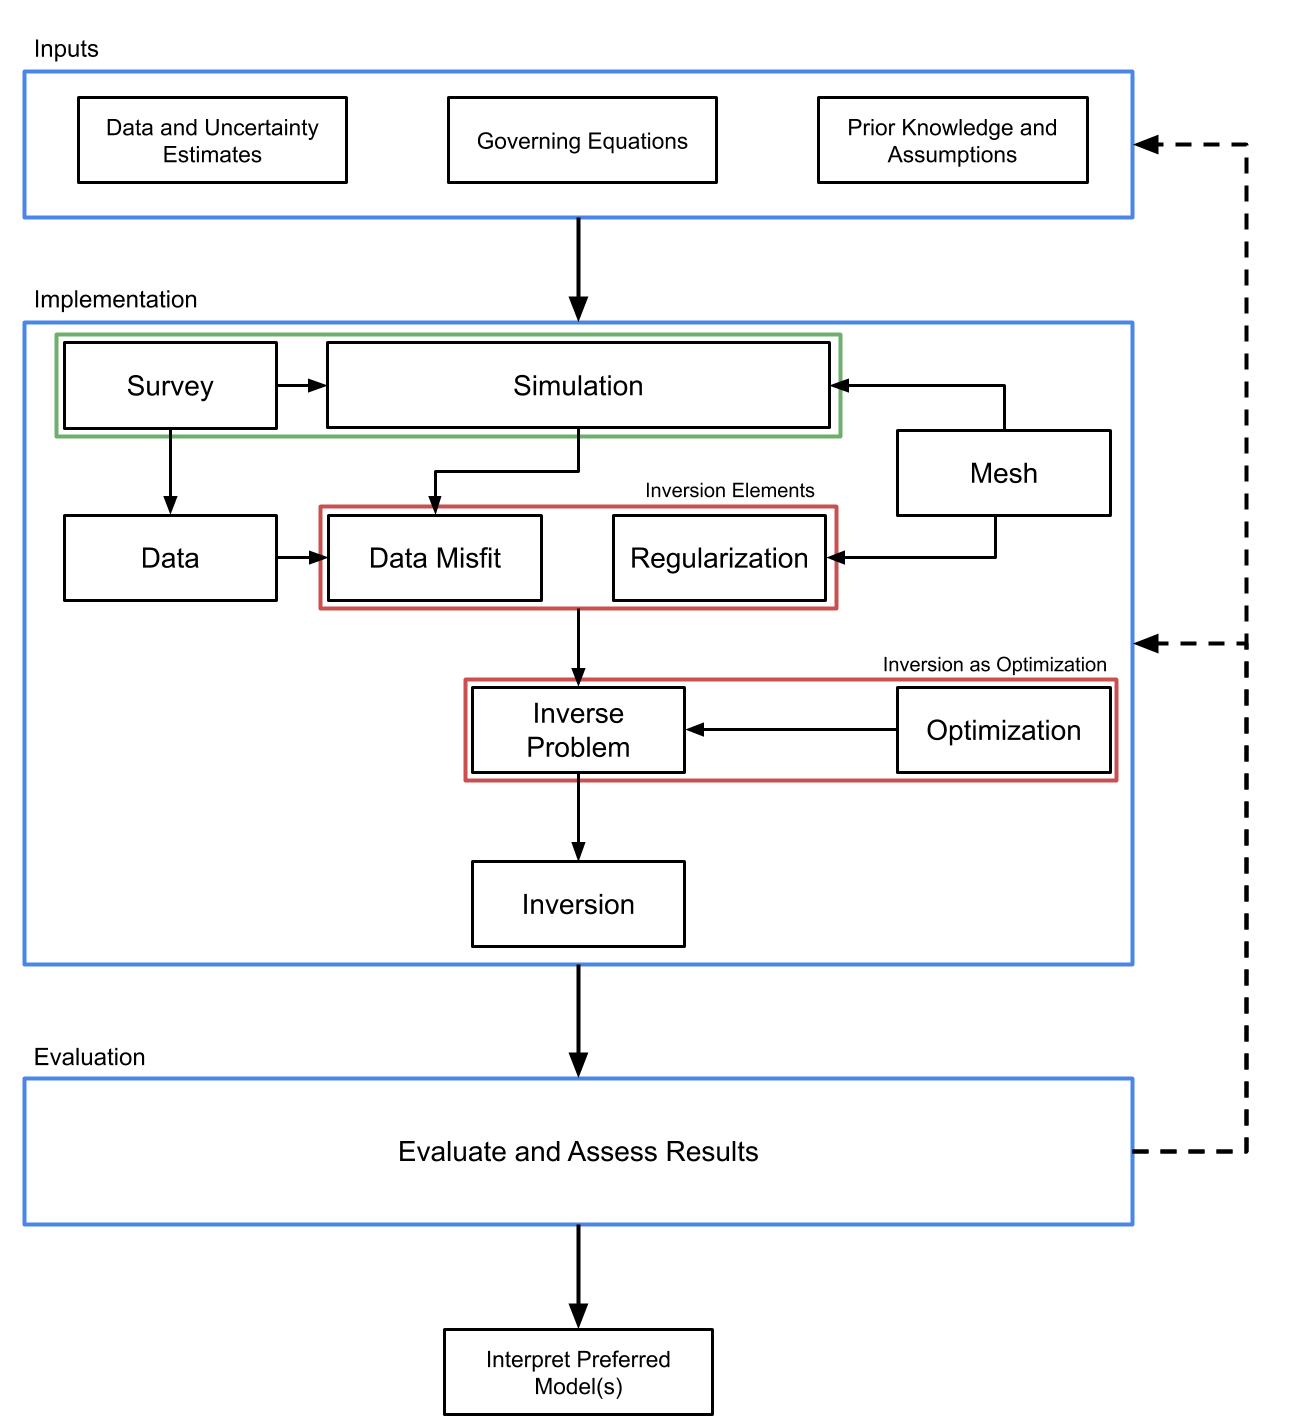
\includegraphics[width=0.8\textwidth]{figures/simpeg-framework.png}
    \end{center}
\caption{
     Framework for solving inverse problems used by SimPEG. After \cite{cockett_simpeg_2015}.
}
\label{fig:simpeg-framework}
\end{figure}


SimPEG's modular framework is common across multiple geophysical techniques; this promotes interactions between researchers having different backgrounds and expertise. Further, it provides an ideal environment for integrating multiple geophysical data sets (e.g. joint inversions) and experimenting with components of the inversion (e.g. regularization).

SimPEG is developed and maintained by a community of contributors that includes graduate students, researchers, and industry professionals. The development follows modern open-source practices including automated testing, code reviews via pull-requests, and discussion about improvements through GitHub issues and in regular open meetings. The combination of the codebase, the community, and the practices adopted by the community are what we refer to as the SimPEG project.

In the following sections, we show three examples from the SimPEG community that were enabled by the open-source nature of the project. The first example illustrates the value of a modular framework by showing the re-use of methods implemented initially for one geophysical method, magnetics, for a different application, time-lapse electromagnetic imaging. The second example discusses joint inversions, which are enabled by having multiple methods implemented in a common framework. The final example shows how research code can be re-purposed for educational and outreach purposes. In each of these examples, ideas have been exchanged, and built upon, more rapidly than would have been possible if the code and community of geoscientists supporting that software were working in isolation.


\subsubsection{Regularization with sparse and compact norms}

The first example we present focuses on the choice of regularization in the inverse problem. As the inverse problem is ill-posed, the regularization plays an important role in allowing us to incorporate existing geologic knowledge and/or assumptions about the model into the inversion.

The regularization term is comprised of a smallness term and first-order smoothness terms that penalize gradients in each of the spatial dimensions, as shown in equation \ref{eq:regularization}.
\begin{equation}
\begin{split}
\phi_m(m) = & \alpha_s \int_V w_s \left| m - m_{\rm ref}\right|^{p_s} dV +
\alpha_x \int_V w_x \left| \frac{\partial m}{\partial x} \right|^{p_{x}} dV + \\
&\alpha_y \int_V w_y \left| \frac{\partial m}{\partial y} \right|^{p_{y}} dV +
\alpha_z \int_V w_z \left| \frac{\partial m}{\partial z} \right|^{p_{z}} dV
\end{split}
\label{eq:regularization}
\end{equation}

The first term is referred to as the ``smallness'' term and penalizes differences between the model ($m$) and a reference model ($m_{ref})$ and the three other terms are often referred to as ``flattness'' or ``first-order'' smoothness terms in the $x, y, z$ directions as they penalize spatial derivatives. The influence of each of these terms in the regularization is weighted by a scalar parameter, $\alpha_{s, x, y, z}$. The $p_{s, x, y, z}$ values indicate the choice of norm. Weights, such as sensitivity weighting, can be applied in the regularization using the $w_{s,x,y,z}$ terms.

A standard inversion uses $\ell_2$-norms (e.g. $p_{s, x, y, z} =2$), resulting in the recovery of smooth structures. The work in \cite{fournier_inversion_2019} develops the approach that is used in SimPEG for solving problems where $p_{s, x, y, z} < 2$. This enables us to recover models with sharp transitions at geologic interfaces and compact structures by promoting sparsity in each term in the regularization. This approach uses iteratively reweighted least squares (IRLS) in performing the optimization. To overcome challenges in optimizing non-convex solutions introduced by using sparse norms ($p_{s, x, y, z} < 2$), this method first seeks an $\ell_2$-norm solution and then finds an $\ell_p$-norm solution.

The initial implementation by \citep{fournier_sparse_2020} was tested on potential fields data collected over the Kevitsa deposit in Finland. The results shown in Figure \ref{fig:sparse-compact-norms-mvi} were obtained from a magnetic vector inversion (MVI) parameterized in spherical coordinates. Regularization is applied to each of the three terms describing the vector magnetization (e.g. repeating equation \ref{eq:regularization} for the amplitude and two angles of magnetization). To promote coherent magnetization directions, an approximate $\ell_0$ norm is applied to the smallness and smoothness terms on the angles of the magnetization. To explore the model space, the norms applied to the amplitude of the magnetization are varied. Figure \ref{fig:sparse-compact-norms-mvi} shows North-South cross-sections through two recovered models at the center of the known nickel deposit. The top image is the result when $\ell_2$ norms are applied to the smallness and smoothness terms on the amplitude while the bottom result shows when an approximate $\ell_0$ norm is applied to the smallness term on the amplitude. Using an approximate $\ell_0$ norm on the orientation and amplitude of the magnetization enables the recovery of more distinct structures, each with a relatively uniform magnetization.

\begin{figure}[!htb]
    \begin{center}
    \includegraphics[width=0.6\textwidth]{figures/sparse-compact-norms-mvi.png}
    \end{center}
\caption{
Cross section through recovered models from MVI inversions that were performed at the Kevitsa deposit in Finland using two different choices of norms \citep{fournier_sparse_2020}. Geological interpretations of a 2D seismic reflection survey are shown in black for reference.
}
\label{fig:sparse-compact-norms-mvi}
\end{figure}


An interesting adaptation of the use of sparse norms was presented by \citep{kang_time-lapse_2022} for time-lapse inversion of airborne electromagnetic data in a saltwater intrusion problem. SkyTEM data were collected in both 2017 and 2019, and the aim is to use both data sets to infer where seawater intrusion may be happening. Performing a 1D spatially-constrained inversion of the 2017 data results in the model shown in the top left of Figure \ref{fig:sparse-compact-norms-aem}; $\ell_2$ norms were applied in the vertical and lateral regularizations. Simply inverting the 2019 data following the same setup and taking the difference between the two recovered models results in the image shown in the top center of Figure \ref{fig:sparse-compact-norms-aem}. However, inversions are non-unique, and without including any additional information, there are many differences between the two models, making it challenging to interpret.

In this work, they also adapt the inverse problem to include a constraint in the time dimension of the form,
\begin{equation}
\phi_t(m) = \alpha_t \int_V w_t \left| \frac{\partial m}{\partial t} \right|^{p_t} dV
\label{eq:time-constraint}
\end{equation}

This equation takes the same form as the first-order smoothness terms in equation \ref{eq:regularization}, but now we are comparing model changes along the time dimension.
Using an $\ell_2$ norm constraint in time results in the image shown in the top right of Figure \ref{fig:sparse-compact-norms-aem}. There are fewer changes between the two years, as a result of imposing the assumption that there should be smooth changes in time.

Hypothesizing that changes of a model value through a time interval (a year) should be sparse, with most of the model remaining constant through time and the changes in conductivity being localized at the saltwater-freshwater interface, the authors impose an approximate $\ell_0$ norm in time. Approximate $\ell_0$ norms are also applied laterally and vertically to promote sharp transitions of conductivity values at the saltwater-freshwater interface. The bottom row of Figure \ref{fig:sparse-compact-norms-aem} shows the recovered models for 2017 and 2019 along with the difference between the two when $\ell_0$ norms are used. By using an approximate $\ell_0$ norm in time, the changes between the two years can be isolated to a few specific areas.  In the recovered model, the difference between the two models is localized to a few specific areas, specifically the red regions near the interpreted freshwater-seawater interface (black line). This may be more realistic in practice and can enable decisions to be made about groundwater management in those areas (e.g., regulating groundwater extraction in those regions).

\begin{figure}[!htb]
    \begin{center}
    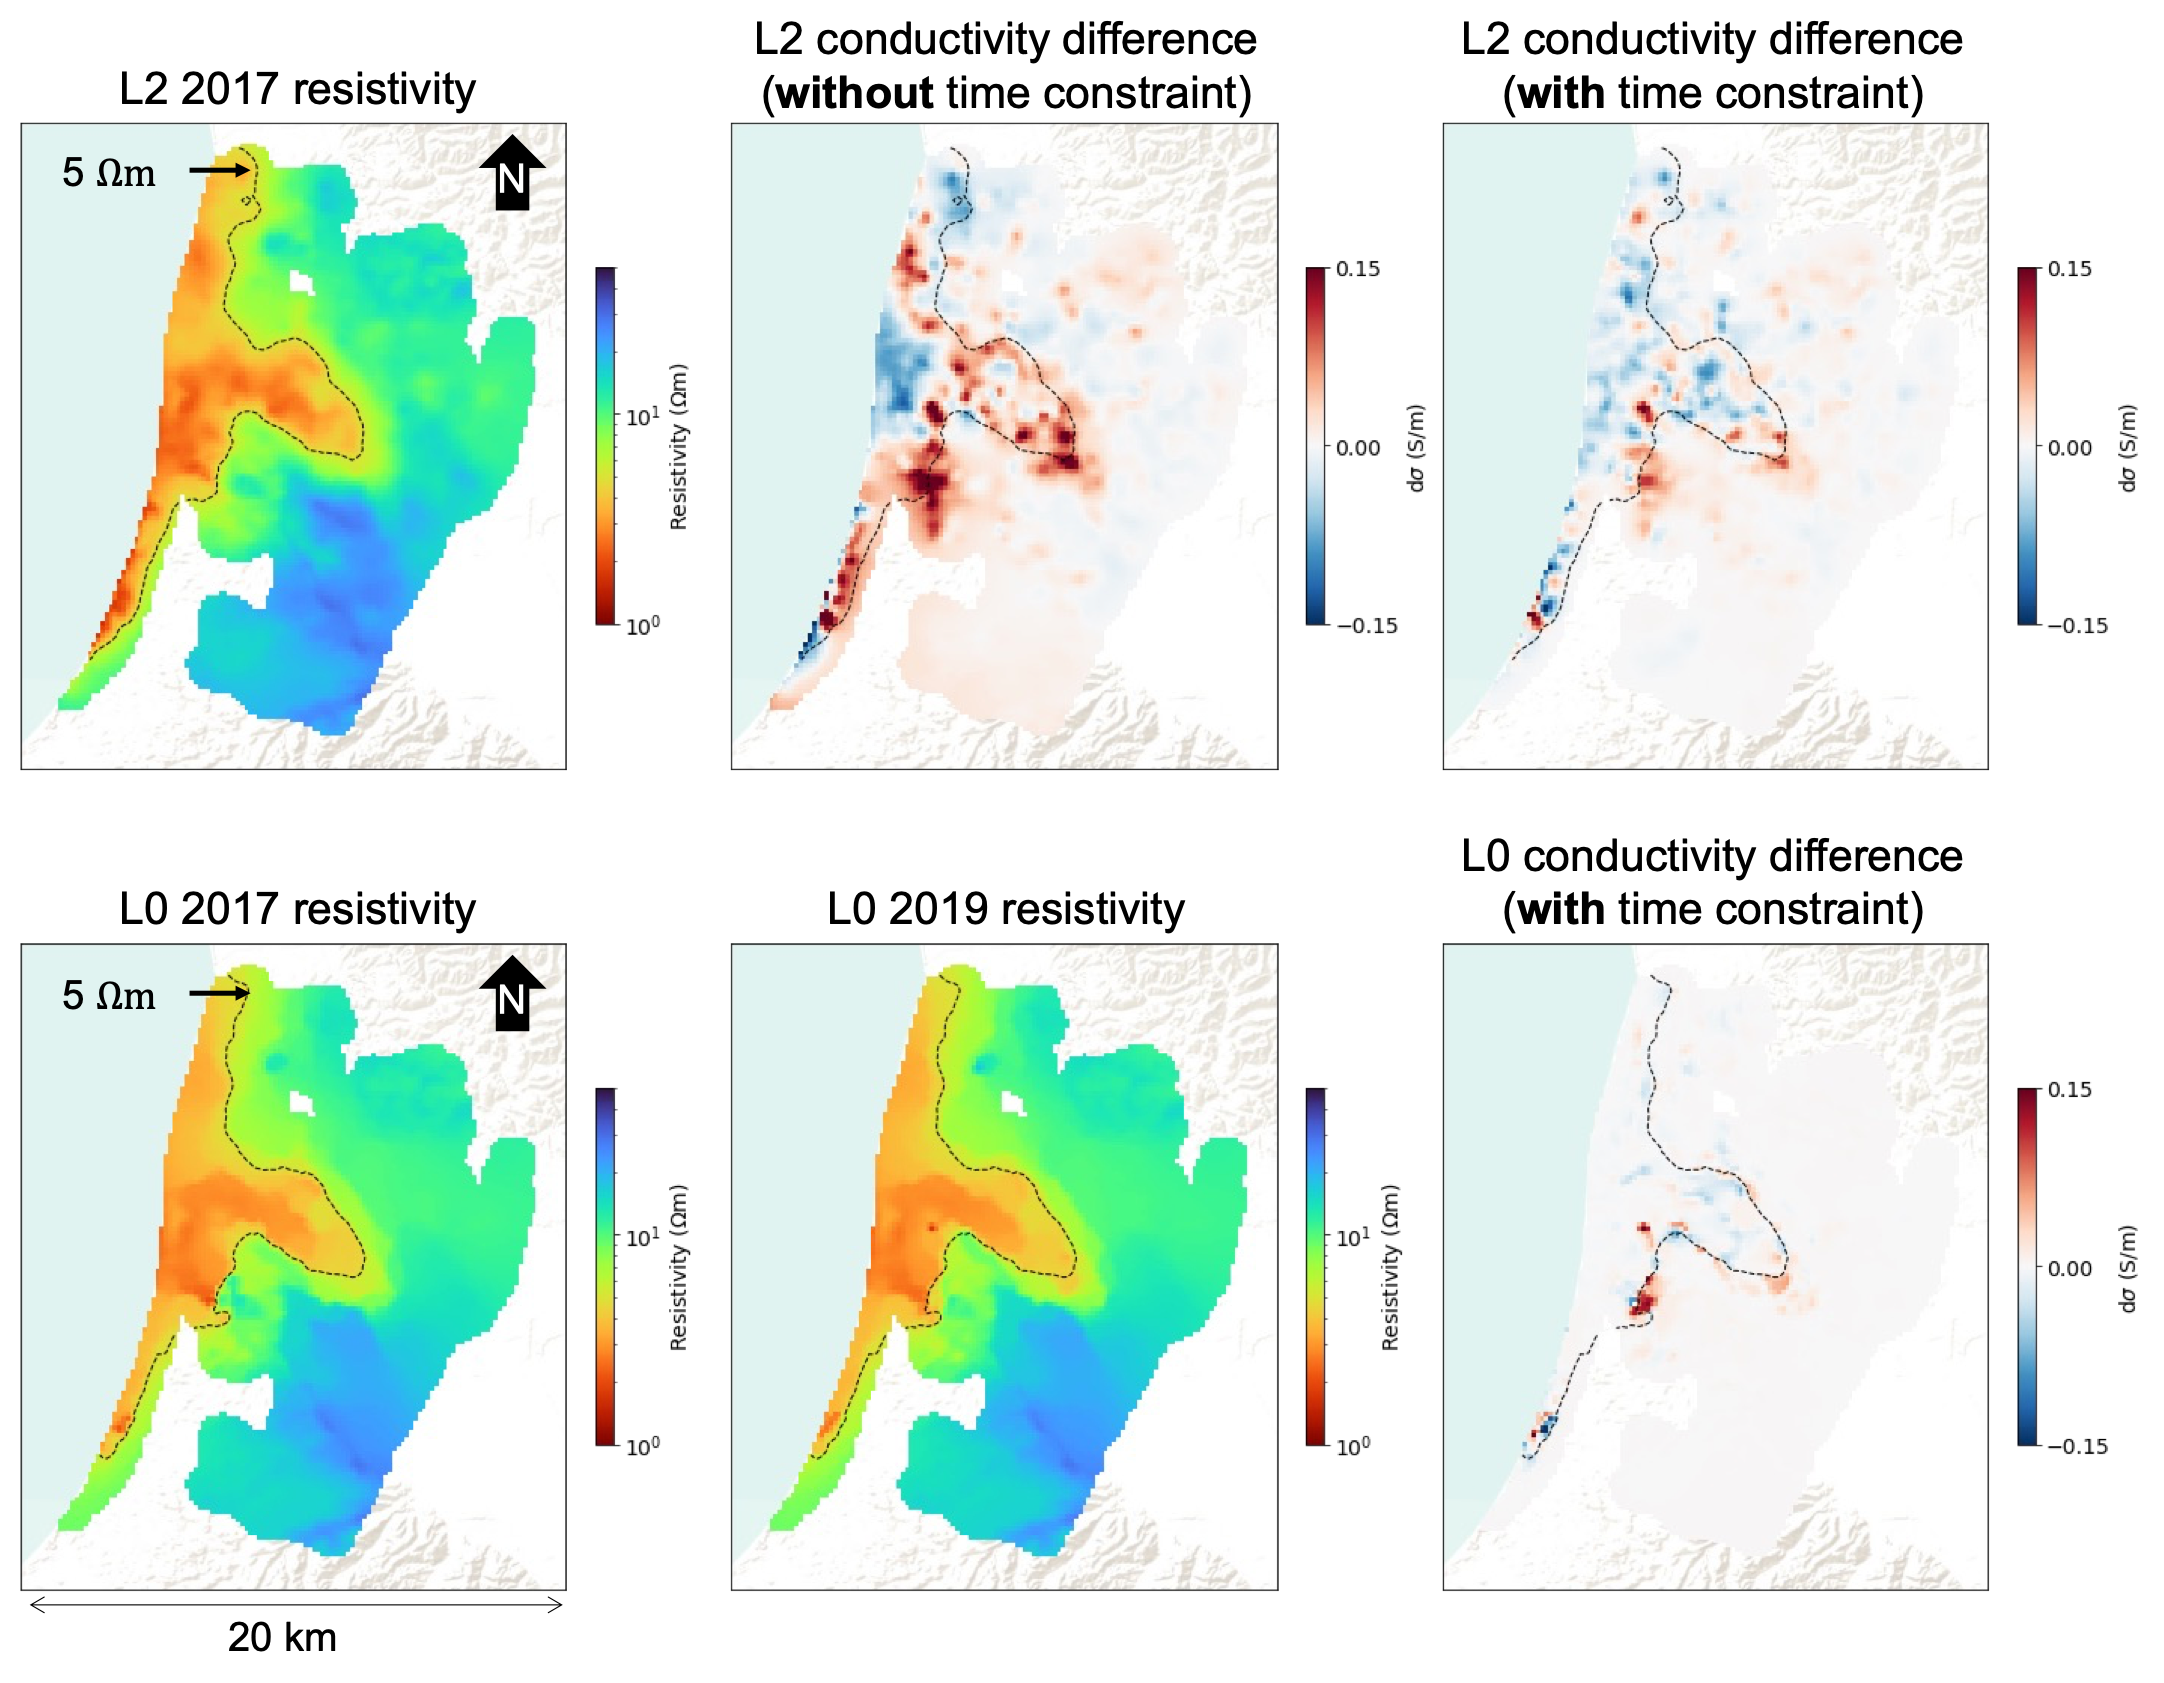
\includegraphics[width=1\textwidth]{figures/time_lapse_resistivity.png}
    \end{center}
\caption{
    Depth slices through inversion results of airborne time-domain electromagnetic data to assess seawater intrusion in California \citep{kang_time-lapse_2022}. The top row shows $\ell_2$ inversion results. The bottom row shows inversion results that make use of sparse and compact norms for both the spatial regularization and the time constraint.The black line on each image is a 5 Ohm-m-contour indicating a potential interface between saltwater and freshwater.
}
\label{fig:sparse-compact-norms-aem}
\end{figure}


In the above magnetic and electromagnetic examples, the same regularization module is used for different geophysical simulations. Adapting from one physics (magnetics) to another physics (electromagnetics) requires the tuning of several hyperparameters in the regularization and IRLS algorithms. In the EM problem, the time constraint is added as a straightforward extension to the regularization. There are also additional complexities since the data are not collected in exactly the same location across the two years. Importantly, this is where a researcher can spend their time and efforts, as opposed to having to re-implement components from scratch as would have been required if the codebases for magnetics and electromagnetics were closed or developed as monoliths. Additionally, the practices in place for peer review, which promotes clarity of code, and documentation, which provides instructions and examples for usage, facilitate more rapid adoption, extension and re-use of ideas implemented in the codebase.



\subsubsection{Joint Inversions}

The next area of research we consider is the joint inversions of multiple geophysical data sets. Given multiple data sets, a common goal is to produce a model of the subsurface that is consistent with all of those data sets. Joint inversions can be a tool for helping solve this problem if an appropriate relationship between the different physical properties and data can be defined. In a general joint inversion, the inverse problem is adapted to include multiple data misfit terms, multiple regularizations, and a coupling term ($\phi_c$) that imposes some similarity measure between the multiple physical property models,


\begin{equation}
\begin{split}
\underset{m}{\text{minimize}} ~ \phi(m) =
\chi_1\phi_{d1}(m_1) + \chi_2\phi_{d2}(m_2) + \beta_1\phi_{m1}(m_1) + \beta_2\phi_{m2}(m_2) + \gamma\phi_c(m_1, m_2)
\\
\quad \text{s.t.}~\phi_{d1} \leq \phi_{d1}^*, \phi_{d2} \leq \phi_{d2}^*
\end{split}
\label{eq:joint-inversion}
\end{equation}


There are different flavors of joint inversions: multiple data sets may be sensitive to the same physical property (e.g. DC resistivity and electromagnetics), or the physical properties that each data set is sensitive to may be distinct. In the latter case, we may then choose a coupling term that imposes some structural similarity, such as cross-gradient (CG) or joint-total variation (JTV) \citep{Gallardo2003, Haber2013}, or a petrophysical constraint, such as fuzzy C-means \citep{Sun2016} or the Petrophysically and Geologically Guided Inversion (PGI) \citep{Astic2019}.

For example, both magnetic and gravity data can be diagnostic in identifying ultramafic rocks with carbon mineralization potential. Ultramafic rocks that have been serpentinized can react with CO$_2$ to produce carbonate minerals. As compared to fresh ultramafic or carbonated units, serpentinized rocks have a low density and generally higher magnetic susceptibility. The works in \citep{capriotti_joint_2023, heagy_geophysical_2022} use synthetic examples to explore the use of joint inversions for delineating serpentinized rocks. Figure \ref{fig:joint-inversion-setup} illustrates the model that is considered. The model has a serpentinized unit (dark green; unit 3), with a central region that has been carbonated (light green; unit 2).

\begin{figure}[!htb]
    \begin{center}
    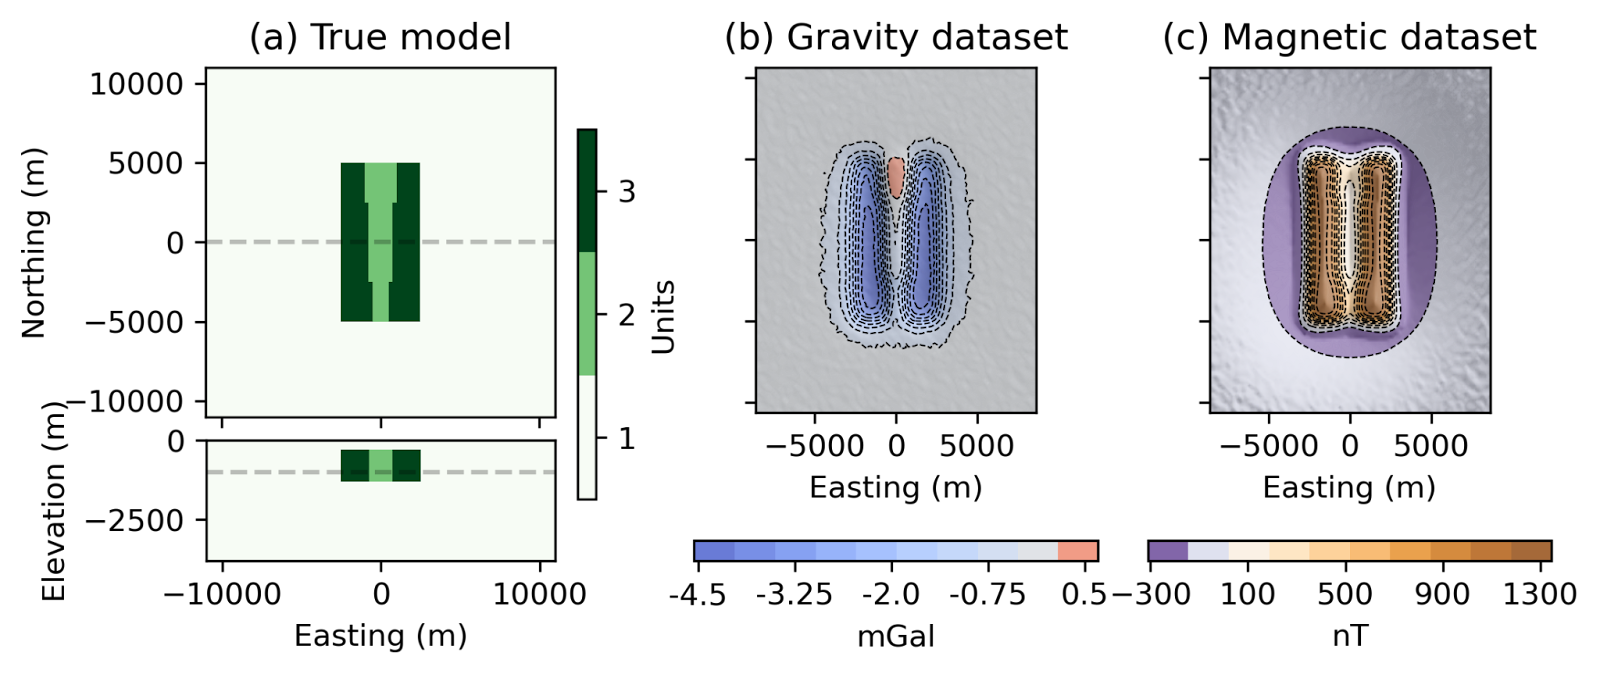
\includegraphics[width=0.95\textwidth]{figures/joint-inversion-setup.png}
    \end{center}
\caption{
    (a) Synthetic model for the carbon mineralization example. The serpentinized unit, unit 3, has a density of 2.7 g/cc,  and 0.15 SI susceptibility.  The carbonated unit, unit 2, has a density of 3.0 g/cc and 0.05 SI susceptibility. The background, unit 1, has a density of 2.9 g/cc and 0 susceptibility. (b) Gravity (c) and magnetic data are simulated on a 19 km by 21 km grid with 250 m grid spacing. After \citep{capriotti_joint_2023}.
}
\label{fig:joint-inversion-setup}
\end{figure}


Figure \ref{fig:joint-inversion} illustrates the use of three different joint inversion approaches for the inversion of gravity and magnetic data in a synthetic example for carbon mineralization \citep{capriotti_joint_2023}. The top row shows: (a) the recovered density model, (b) the recovered susceptibility model, and (c) a cross-plot of the recovered physical properties for a cross-gradient inversion. The stars in (c) show the physical properties corresponding to the three rock units from Figure \ref{fig:joint-inversion-setup}. The second and third rows show joint inversion results using joint total variation and the petrophysically and geologically guided inversion (PGI), respectively. Each of the joint inversion approaches promotes different structures and features in the physical property cross-plots. Cross-gradient promotes co-located non-zero gradients in the model, and in the physical property cross plot, we can see that it promotes linear features. Joint total variation promotes joint sparsity (e.g. having non-zero values located in the same spatial location). PGI promotes clusters in physical property space. Each approach has advantages and settings where it is more or less well-suited for the problem, but being able to compare multiple strategies enables us to build confidence in common features of the models and also to understand the features one approach tends to promote.


\begin{figure}[!htb]
    \begin{center}
    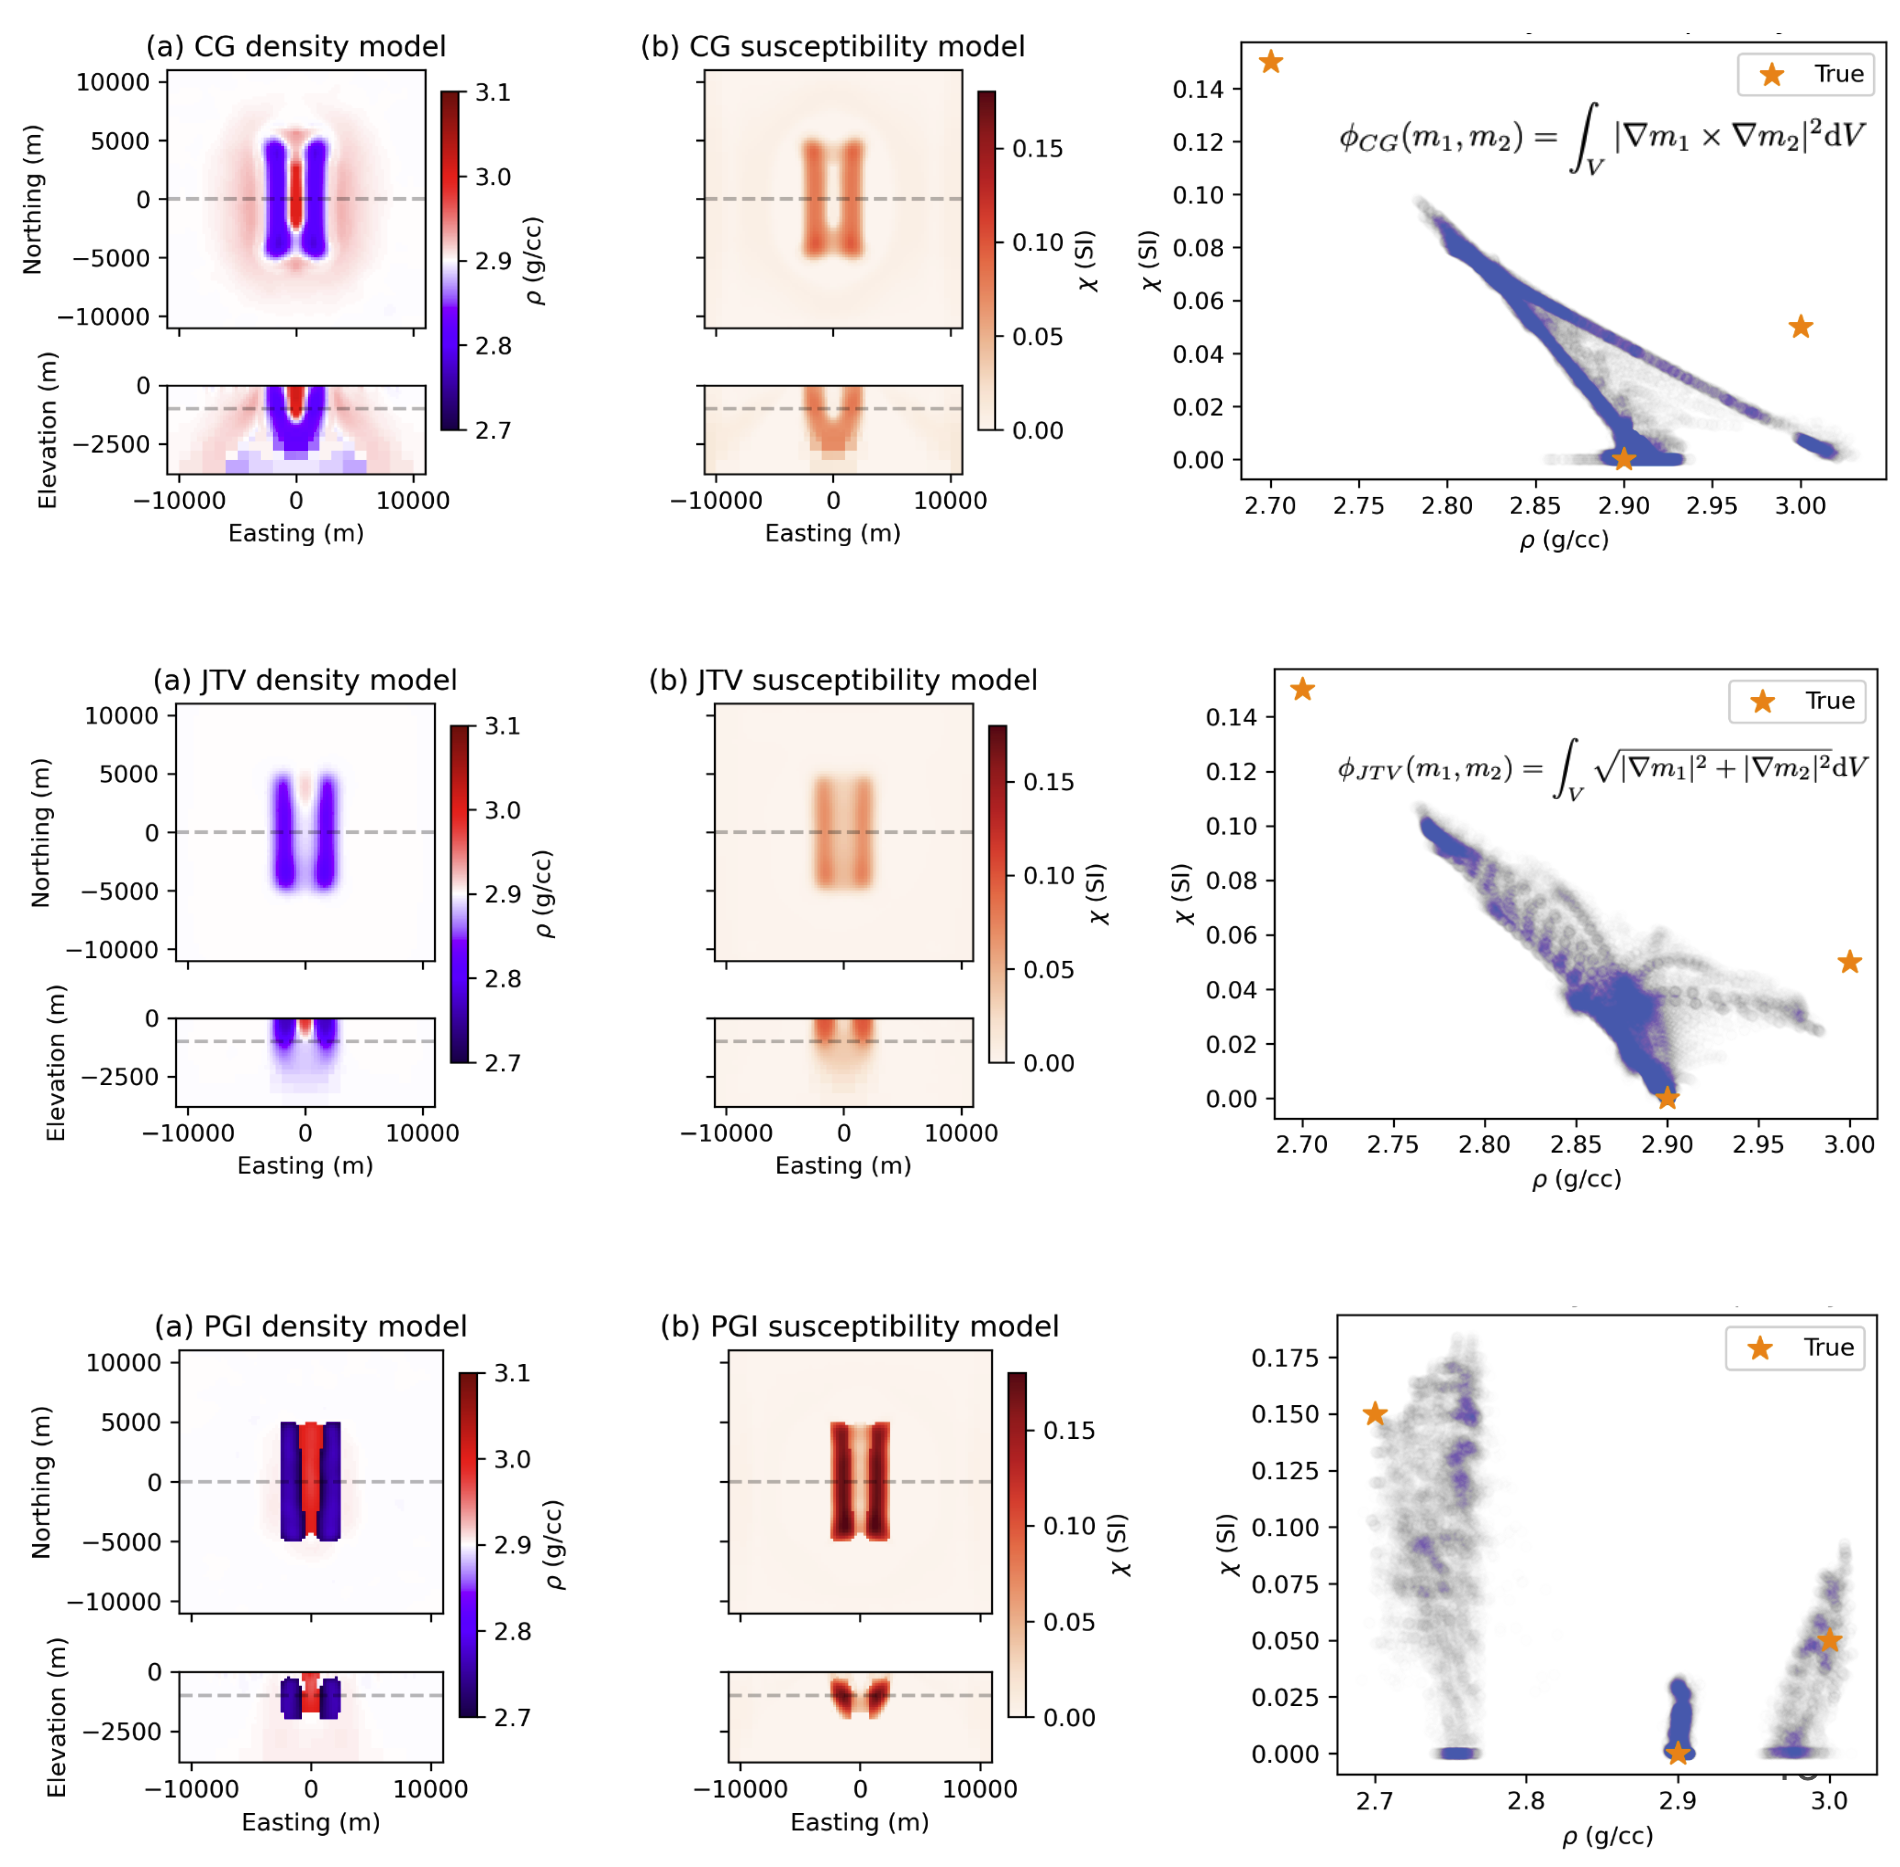
\includegraphics[width=0.95\textwidth]{figures/joint-inversion.png}
    \end{center}
\caption{
    Joint inversions of synthetic gravity and magnetic data for a carbon mineralization application. The central unit of carbonated rock (high density and moderate susceptibility) is embedded in a serpentinized unit (low density and high magnetic susceptibility). After \citep{capriotti_joint_2023}.
}
\label{fig:joint-inversion}
\end{figure}


Having a common framework for each physical simulation provides the components for implementing a joint inversion. In SimPEG, to form a combined data misfit, the user simply creates each data misfit term as they would for individual inversions and sums them together (e.g. \texttt{phi\_d = chi\_1 * phi\_d1 + chi\_2 * phi\_d2}). There are a number of practical challenges in obtaining a good result from a joint inversion, including choosing a coupling term, weighting each of the terms in equation \ref{eq:joint-inversion} appropriately, and designing a strategy for updating parameters as the inversion runs to fit each of the data sets adequately. These are non-trivial and require experimentation by the user. But prior to being able to experiment with approaches, all of the necessary components including the OcTree mesh and operators, implementation of each of the forward simulations, the optimization machinery, etc., must be in place. Each of these components requires different skills and expertise and development can be accelerated through collaborations amongst researchers with different skill sets. In fact, generating the results shown in Figure \ref{fig:joint-inversion} required the use of code written by 10 different people from 4 different academic and industry institutions. Each contributor to this collaborative project brings their own goals and interests. This scale and style of organic collaboration is possible when researchers derive value from and choose to invest efforts in a common set of open-source tools.


\subsubsection{Education and outreach}

The final area we discuss is the role of educational resources in promoting the use of geophysics. In many cases, the decision to use geophysics (or not) for a given application is made by an engineer, a manager, or someone else who is not themselves a geophysicist. Resources that illustrate the use of geophysics and fundamental concepts about the various geophysical methods can be useful tools for communicating the role that geophysics can play in helping solve an applied problem.

In our experience, we have found that using simulations and enabling others to change various input parameters and visualize outputs has been an impactful way to illustrate fundamental concepts. For the 2017 SEG Distinguished Instructor Short Course (DISC), we developed a collection of Jupyter Notebook ``Apps'' where users can interact with simulations based on SimPEG through widgets (e.g. slide bars, toggle buttons, etc) \citep{Oldenburg2021}. Similarly, we designed Notebook-Apps for a Geoscientists Without Borders (GWB) project aimed at using DC resistivity to decide where to drill for groundwater in Mon State Myanmar \citep{fan2020improving}. We created two styles of apps. The first collection of apps was aimed at facilitating understanding of fundamental concepts, such as how the presence of a conductive or resistive layer alters the flow of currents and therefore the measured potentials at the surface of the earth. The second collection of apps provides template workflows for loading, visualizing and inverting data to obtain a resistivity model using SimPEG. An example of one of the apps is shown in Figure \ref{fig:jupyter-apps}.



\begin{figure}[!htb]
    \begin{center}
    \includegraphics[width=1\textwidth]{figures/jupyter-apps.png}
    \end{center}
\caption{
    Participants in Mon State Myanmar using Jupyter Notebook ``Apps'' to explore fundamental concepts of DC resistivity as a part of a 2019 Geoscientists Without Borders project \citep{fan2020improving}.
}
\label{fig:jupyter-apps}
\end{figure}


An additional benefit of building educational resources on top of open-source research tools is that these resources can provide an on-ramp for participants to use these tools in their own work. For the GWB project, participants used these notebooks to identify more than 20 locations to drill for groundwater after the North American team left Myanmar. Educational uses of the SimPEG software have also led to improvements in the code base, for example, efficiency improvements were made to the DC resistivity code as described in \cite{Kang2020} to support geoscientists running inversions on older laptops with limited RAM. These improvements are equally valuable for inverting large-scale datasets. Having a common set of tools and resources where research code is re-purposed for education, and visa-versa, drives improvements that benefit both use cases. Importantly, it also provides avenues for ``students'' to become contributors.



\subsection{Some takeaways}

These three examples illustrate how open-source software can enable collaboration, facilitate the exchange and extension of ideas, and promote the use of geophysics to help solve applied problems. In our experience, these examples may not have been possible, or would have required substantially more time and effort, without open-source software and communities. In particular, the use of a permissive license has been key for promoting engagement and contributions from geoscientists in industry as code with a permissive license can be included in commercial products. These connections drive improvements and use in new applications by industry practitioners.

In addition to the licensing terms, SimPEG is a project supported by a community of contributors and the set of open-source practices used in this community have implications on its growth and impact. For example, having comprehensive tests for the codebase enables collaborations; it allows others to propose improvements to the code without the fear of breaking it. ``Pull requests'' facilitate peer review of code; this process can help catch unhandled edge cases that the original author may not have considered or result in changing the names of variables for clarity and maintainability of the code. Documentation and tutorials help users get started with the code, and online forums and meetings provide a space for discussion about both the software and the scientific problems it is being used to address. These components of social infrastructure are key for scalable collaboration.

Relationships and partnerships between industry and academic groups are also evolving in light of the shift to open-source. Much research has been funded under a model where companies sponsor research groups that produce software that is proprietary to sponsors. An open-source model has several advantages compared to a closed-source sponsorship. Research and development are conducted in the same project where ``production’' code is deployed, reducing the time and effort necessary for technology transfer. It also opens new opportunities for collaboration between industry practitioners and academic researchers as both groups can suggest changes to the code and make improvements as it is used. Importantly, highly qualified scientists are trained in developing and contributing to the same codebase that they will use in their careers. Our experience has shown that there is now a critical mass of industry partners who see value in these aspects and are willing to support this model of partnership going forward.

There are now many open-source projects in geophysics following similar practices and solving common problems. There is some overlap between the scope and purpose of projects. Although this could be viewed as a duplication of efforts, we view this as an advantage, particularly for complex problems because different groups take different approaches and handle some implementation details differently. Studies that compare solutions can help build confidence in a result and differences can be investigated when code is available. For example, works such as \cite{Werthmuller2020} compare forward simulations of the 3D Maxwell's equations, and \cite{doyoro_review_2022} compare DC resistivity inversion results between four different inversion codes. These types of comparisons are valuable resources for building confidence in different codebases and illustrating where differences in the details of a given approach impact the results.

We often refer to an open-source project existing within an ``ecosystem,'' referring to a collection of projects that are interconnected and can build upon each other. For example, SimPEG relies upon several core scientific Python packages and leverages external packages for high-performance computing such as Dask and Numba. There are several advantages to this modular, interoperable ecosystem model: it allows for the separation of concerns amongst the various projects so each can remain scoped, and when improvements are made in one project, all groups that rely on that project benefit from those advancements. Improvements in performance and efficiency of code are natural examples. Additionally, when we consider the broader research landscape, an ecosystem model allows us to interoperate with advancements made in other fields. There is much potential and value already being derived from the use of open-source software in machine learning. For example, the Petrophysically and Geologically Guided Inversion approach discussed earlier relies upon tools in the scikit-learn package \cite{Pedregosa2011} which has tools for classic machine learning. Tools for deep learning such as PyTorch and Tensorflow exist within the same ecosystem. Combining methods from ML and deep learning with geophysical methods is an area ripe for innovation and exploration and this is aided by having accessible, interoperable tools.

\section{Looking to the future}

Many of the practices from open-source can be applied at different scales and different stages of research. Not every research project should turn into an ``open-source package'' that is maintained over time. However, the practice of sharing code promotes transparency, enables deeper conversations about the methods employed, and facilitates reuse and extensions of work. This is true even for unpolished code. In our experience, planning to share code alongside a publication has also prompted better software practices such as improving variable names or reducing duplicate code, because we know our peers may look at it. This positive social pressure can promote the development of more reliable research code.

Beyond software, open communication of science broadens conversation to ``open science.'' \cite{unesco_introduction_2023} defines open science as \emph{a set of principles and practices that aim to make scientific research from all fields accessible to everyone for the benefits of scientists and society as a whole.} An emphasis in the UNESCO recommendations is that research be ``as open as possible,'' recognizing that there are scenarios where access to data or intellectual property may need to be restricted. In addition to software, open science encompasses ideas such as the FAIR principles for data (FAIR: findable, accessible, interoperable, reusable), and sharing publications in an openly accessible way, for example posting pre-prints of publications on servers such as ArXiv or Earth ArXiv. Taking steps to make research outputs accessible facilitates transparency, reproducibility, and ultimately extension of ideas. These concepts are core to how science progresses.

In this paper, we illustrated the role of open-source software and practices in three examples: reusing regularization methods with different geophysical surveys, combining simulations to perform joint inversions, and repurposing research code for use in educational and humanitarian projects. Re-use and extension are enabled because the code is freely available for use and adaptation, and importantly because the set of practices around development and communication facilitates collaboration amongst a community of researchers with different backgrounds, skill sets, and interests. Having input and contributions from multiple people with different strengths accelerates development. Having the developed methods applied to a variety of applied problems and in a range of contexts, including research, education, and industrial applications, improves reliability and robustness, which in turn allows further reuse in other domains.

The applications where geophysics can make a positive impact in society are complex and require data, knowledge, and methods from multiple disciplines. We have experienced how open science practices have facilitated rapid re-use and extension of work and enabled the types of collaborations across disciplines that are necessary for solving complex problems. These open science practices are most effective when adopted by a community of researchers and practitioners. Such a community will have immense potential to accelerate the use and effectiveness of geophysics in helping to reach solutions to the complex geoscientific problems society faces.

\section{Acknowledgment}

The authors are grateful to Dr. Yaoguo Li and Dr. Michael Wilt for organizing this special issue and for their feedback on an earlier version of the manuscript. We thank the one anonymous reviewer who provided constructive feedback on our manuscript. We are also grateful to members of the SimPEG community for their contributions to the codebase and culture of the community.
